\documentclass[tikz,border=8pt]{standalone}
\usetikzlibrary{arrows.meta,positioning,fit,calc}
\begin{document}
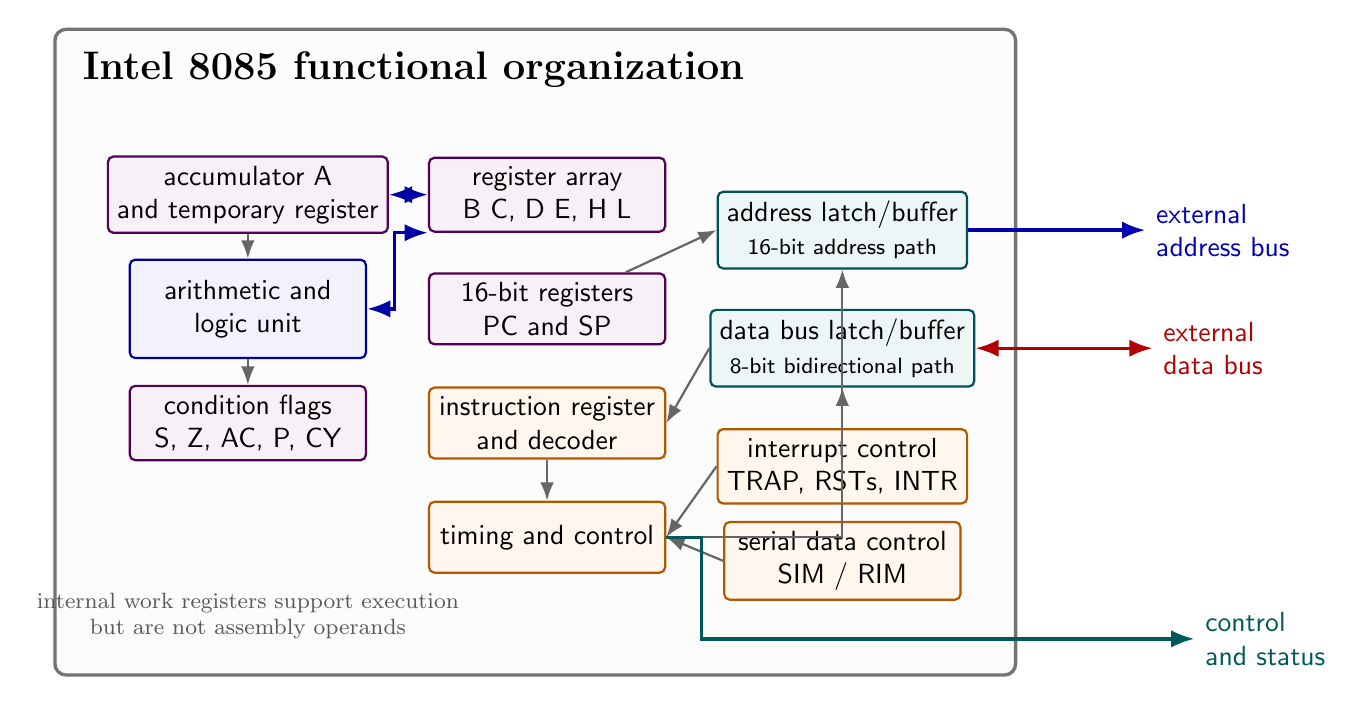
\begin{tikzpicture}[
  font=\sffamily,
  >=Latex,
  block/.style={draw=blue!60!black,rounded corners=2pt,thick,minimum width=3.0cm,minimum height=.9cm,align=center,fill=blue!5},
  reg/.style={block,draw=violet!65!black,fill=violet!6},
  ctl/.style={block,draw=orange!70!black,fill=orange!7},
  ext/.style={block,draw=teal!65!black,fill=teal!7},
  bus/.style={<->,very thick,blue!65!black},
  flow/.style={->,thick,black!60}
]
  \node[draw=black!55,rounded corners=4pt,very thick,minimum width=12.2cm,minimum height=8.2cm,fill=black!1] (chip) at (0,0) {};
  \node[font=\bfseries\Large,anchor=north west] at ([xshift=.25cm,yshift=-.18cm]chip.north west) {Intel 8085 functional organization};

  \node[reg] (acc) at (-3.65,2.0) {accumulator A\\and temporary register};
  \node[block,minimum height=1.25cm] (alu) at (-3.65,.55) {arithmetic and\\logic unit};
  \node[reg] (flags) at (-3.65,-.9) {condition flags\\S, Z, AC, P, CY};

  \node[reg] (gp) at (.15,2.0) {register array\\B C, D E, H L};
  \node[reg] (pcsp) at (.15,.55) {16-bit registers\\PC and SP};
  \node[ctl] (decode) at (.15,-.9) {instruction register\\and decoder};
  \node[ctl] (timing) at (.15,-2.35) {timing and control};

  \node[ext] (addr) at (3.9,1.55) {address latch/buffer\\\footnotesize 16-bit address path};
  \node[ext] (data) at (3.9,.05) {data bus latch/buffer\\\footnotesize 8-bit bidirectional path};
  \node[ctl] (intr) at (3.9,-1.45) {interrupt control\\TRAP, RSTs, INTR};
  \node[ctl] (serial) at (3.9,-2.65) {serial data control\\SIM / RIM};

  \draw[bus] (acc) -- (gp);
  \draw[flow] (acc) -- (alu);
  \draw[flow] (alu) -- (flags);
  \draw[bus] (alu.east) -- ++(.35,0) |- (gp.south west);
  \draw[flow] (pcsp) -- (addr.west);
  \draw[flow] (data.west) -- (decode.east);
  \draw[flow] (decode) -- (timing);
  \draw[flow] (intr.west) -- (timing.east);
  \draw[flow] (serial.west) -- (timing.east);
  \draw[flow] (timing.east) -| (addr.south);
  \draw[flow] (timing.east) -| (data.south);

  \draw[->,very thick,blue!70!black] (addr.east) -- ++(2.25,0) node[right,align=left]{external\\address bus};
  \draw[<->,very thick,red!70!black] (data.east) -- ++(2.25,0) node[right,align=left]{external\\data bus};
  \draw[->,very thick,teal!70!black] (timing.east) -- ++(.45,0) |- ([yshift=.48cm]chip.south east) -- ++(2.25,0) node[right,align=left]{control\\and status};

  \node[font=\footnotesize,text=black!65,align=center] at (-3.65,-3.35) {internal work registers support execution\\but are not assembly operands};
\end{tikzpicture}
\end{document}
